%!TEX root = ../main.tex

\section{Введение}

\begin{frame}{Физическое явление}
\begin{block}{Электрический пробой}
	Явление резкого возрастания тока в диэлектрике при приложении электрического напряжения
	выше критического.
\end{block}
\begin{itemize}
	\item Рассматриваем твердый диэлектрик
	\item Деградация диэлектрических свойств материала
	\item Процесс развивается в ограниченной зоне -- канале пробоя
	\item Сложная физическая природа
\end{itemize}
\end{frame}


\begin{frame}{Математическая модель}
\begin{block}{Модель типа диффузной границы}
	Вещество находится в разных фазах. Состояние вещества описывается гладкой функцией
	$\phi(\vx, t)$ -- фазовым полем.
\end{block}
\begin{itemize}
	\item $\phi = 1$ -- неповрежденная среда
	\item $\phi = 0$ -- полностью разрушенная среда
	\item Зона $\phi \in (0, 1)$ -- диффузная граница
	\item На разрушение среды тратится энергия
\end{itemize}
\begin{figure}
	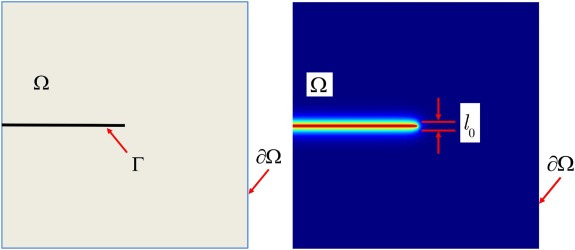
\includegraphics[width=0.5\textwidth]{figures/diffuse_edge.jpg}
\end{figure}
\end{frame}


\begin{frame}{Математическая модель}
Модель, предложенная в работе \cite{pitike_dielectric_breakdown}:
\begin{itemize}
	\item $\pi = \textcolor{red}{-\half \epsilon[\phi] (\nabla \Phi, \nabla \Phi)} +
	\Gamma \left( \cfrac{1 - f(\phi)}{l^2} + \cfrac{1}{4} (\nabla \phi, \nabla \phi) \right)$
	-- плотность свободной энергии
	\item $\Gamma$ -- энегрия роста канала пробоя на единицу длины
	\item $l$ -- величина <<размытия>> канала
	\item $\epsilon(\vx, t)$ -- диэлектрическая проницаемость среды
	\item $f(\phi)$ -- интерполирующая функция
\end{itemize}
\end{frame}


\begin{frame}{Математическая модель}
\vspace{-0.2cm}
\begin{itemize}
	\item $\epsilon(\vx, t) = \cfrac{\epsilon_0(\vx)}{f(\phi(\vx, t)) +
	\delta}$ -- диэлектрическая проницаемость среды
	\item $f(\phi) = 4 \phi^3 - 3 \phi^4$ -- интерполирующая функция
\end{itemize}
\begin{columns}
\column{0.5\textwidth}
\begin{figure}
	\hspace*{1.4cm}
	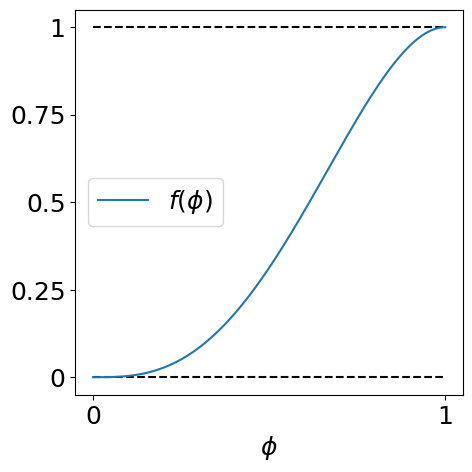
\includegraphics[width=0.65\textwidth]{figures/f_form.png}
\end{figure}
\column{0.5\textwidth}
\begin{figure}
	\hspace*{-2cm}
	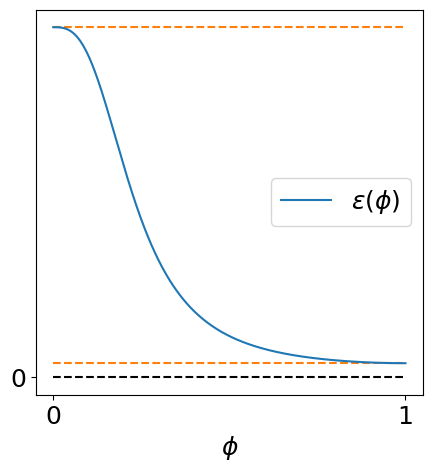
\includegraphics[width=0.60\textwidth]{figures/eps_form.png}
\end{figure}
\end{columns}
\end{frame}


\begin{frame}{Математическая модель}
\vspace{-0.5cm}
\begin{block}{Уравнения модели}
\begin{itemize}
	\item Уравнение электрического потенциала $\Phi$:
	\begin{equation}
		\Div(\epsilon[\phi] \nabla \Phi) = 0
		\label{equation_potential}
	\end{equation}
	\item Уравнение фазового поля $\phi$:
	\begin{equation}
		\cfrac{1}{m} \partt{\phi} = \half \epsilon'(\phi) \gradscalsq{\Phi} + \cfrac{\Gamma}{l^2} f'(\phi) + \half \Gamma \Delta \phi
		\label{equation_phase}
	\end{equation}
\end{itemize}
\end{block}
Свойства:
\begin{itemize}
	\item связанная система уравнений на $\phi$ и $\Phi$;
	\item уравнение для $\phi$ типа Аллена--Кана, нелинейное.
\end{itemize}
\end{frame}


\begin{frame}{Пример вычислительного эксперимента}
\begin{columns}
\column{0.32\textwidth}
\begin{figure}
	
\includegraphics[width=\textwidth]{figures/model_example_1.png}
\end{figure}
\column{0.32\textwidth}
\begin{figure}
	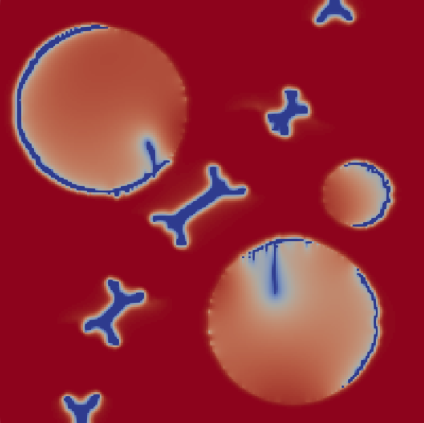
\includegraphics[width=\textwidth]{figures/model_example_2.png}
\end{figure}
\column{0.32\textwidth}
\begin{figure}
	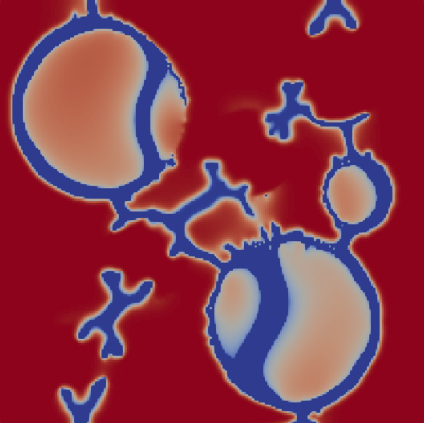
\includegraphics[width=\textwidth]{figures/model_example_3.png}
\end{figure}
\end{columns}
\begin{center}
	Расчет из работы \cite{zipunova_experiment}
\end{center}
\end{frame}


\begin{frame}{Цель работы}
\begin{block}{Цель работы}
	Исследовать качественные характеристики системы уравнений \eqref{equation_potential},
	\eqref{equation_phase} и выполнить ее численный анализ.
\end{block}
Для этого рассмотрим задачу в определенных краевых условиях, упрощающих ее, но позволяющих
установить интересующие свойства.
\end{frame}